\subsection{Loss functions}
The problem of decoy quality assessment is essentially a ranking
problem: we have to arrange decoys according to their similarity to
the corresponding native structure, as quantified by the GDT\_TS score
\cite{zemla2001casp4}, for instance. Such a ranking approach to the
problem of model quality assessment has recently been used by the
MQAPRank method \cite{jing2016sorting}, which, however, relies on a
support vector machine architecture and uses high-level features as
input.

In the present work, we define the loss function in terms the margin
ranking loss for each pair of decoys. Let a decoy representation be
denoted as $x_i$ and the output of the network for this decoy as
$f(x_i)$. Let $y_{ij}$ be the ordering coefficient of the two decoys:
$$
y_{ij} = \begin{cases}
               1& \text{if }\text{GDT\_TS}_i \leq \text{GDT\_TS}_j \\
               -1& \text{if }\text{GDT\_TS}_i > \text{GDT\_TS}_j \\
            \end{cases}
$$
%
Here, $\text{GDT\_TS}_i$ is the global distance test total score of
the $i$-th decoy. We use the following expression for the pairwise
ranking scoring function:
$$
L_{ij} = w_{ij} \cdot \max \left[ 0, 1 - y_{ij} \left( f \left( x_i \right) - f \left( x_j \right) \right) \right]
$$
%
The term $w_{ij}$ represents an example weight:
%
$$
w_{ij} = \begin{cases}
               1& \text{if } \left| \text{GDT\_TS}_i - \text{GDT\_TS}_j \right| > T \\
               0& \text{otherwise} \\ 
            \end{cases}
$$
%
where $T$ is a threshold constant set to 0.1~{\AA}. This has the
effect of avoiding to train the model on pairs of decoys that are too
similar.

During the training procedure we load $N_\text{B}$ decoy structures of
a given target into memory (a ``batch'') and compute the output of the
network and the average loss:
$$ L = \frac{1}{N^{2}_\text{B}} \sum_{i=1,j=1, i \neq j}^{N_\text{B}} L_{ij} $$
Afterwards, we compute the gradient of the average loss with respect
to the network parameters and update them using the Adam algorithm
\cite{kingma2014adam}. We use a batch size $N_B = 9$.


\subsection{Evaluation criteria}
We evaluate the model using various correlation coefficients of the
scores and using a loss criterion defined, for any given protein, as
the absolute difference between the GDT\_TS of the best decoy and the
GDT\_TS of the decoy with the lowest $f$ score:
$$ 
\text{Loss} = \left| \max_i( \text{GDT\_TS}_i ) - \text{GDT\_TS}_{\mathrm{argmin}_i(f(x_i))} \right|
$$
%
The correlation coefficients between the $f$ score produced by the
model and the GDT\_TS score are computed for all decoys of a given
protein in the test set, and are then averaged over all
proteins. Since the value of GDT\_TS increases with the quality of a
model but the value of $f$ decreases, an ideal model would show a
correlation coefficient of $-1$.


\subsection{Optimization and dataset sampling}
The optimization of the parameters of our model was performed
using the the Adam algorithm \cite{kingma2014adam}. The gradient of the loss 
function with respect to the model parameters was computed on the pairs of 
models in the batch. The batch size was set to $M = 9$ models.
%%%
%%% GL: This paragraph needs some work
%%%
%G: Rewrote this paragraph


The training dataset is sampled in the following way: first we choose a
random target from the dataset, then we sample decoys of this
target. One epoch corresponds to one pass through all targets in the
dataset. The decoys are sampled in a homogeneous way: we divide all
the decoys into $M = 9$ bins by the value of GDT\_TS score.
Precisely, the decoy $i$ belongs to the bin number $ \left[
  \frac{\max(\text{GDT\_TS}) - \text{GDT\_TS}_i}{\max(\text{GDT\_TS})
    - \min(\text{GDT\_TS})} \right] + 1$, where $\max(\text{GDT\_TS})$
and $\min(\text{GDT\_TS})$ are computed for all the decoys of the
chosen protein. If there are empty bins, then we take second decoy
from each non-empty and so on until we filled the batch. At the end
of each epoch we randomly shuffle the order of targets and the order
of decoys in each bin.

Decoy structures are randomly rotated and translated each time they
are used as input. The rotations are sampled uniformly
\cite{shoemake1992uniform} and the translation are chosen in such a
way that the translated protein fits inside the $120$~\AA${}\times
120$~\AA${}\times 120$~\AA\ input grid.
%%% GL: Do you add a buffer so that the *density* of the protein also
%%% fits inside the grid? In other words, do you prevent any atom from
%%% being less than 2 Angstroms away from the edges of the grid?
%G: It is a minor detail, we will release the source-code, so not mentioning it 
%is not an issue, imho.

We select the final model based on its performance on a
\emph{validation subset} consisting of 35 targets (and their decoys)
picked at random from the training set and excluded from the training
procedure. The remaining 529 targets are called the \emph{training
subset}.  Figure~\ref{Fig:TrainingLoss} shows the Kendall $\tau$ and
Pearson $R$ coefficients and the loss on the validation subset over 52
epochs of training.  Models are saved every 10 epochs and we pick the
one that has the smallest loss (at epoch 40).

\begin{figure}[H]
    \centering
    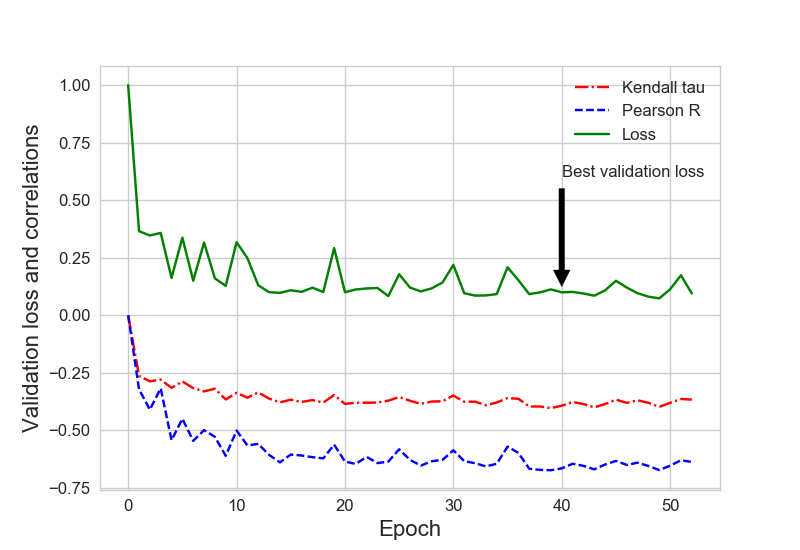
\includegraphics[width=\linewidth]{Fig/kendall_validation.eps}
%
    \caption{Loss, Kendall $\tau$, and Pearson $R$ coefficients
      evaluated on the validation subset during the training
      procedure.  One epoch corresponds to a cycle over all targets in
      the training subset. Models are saved every 10 epochs and the
      arrow shows the minimum validation loss for which a model was
      saved (at epoch 40).}
%
    \label{Fig:TrainingLoss}
\end{figure}

Table \ref{Tbl:TrainingResults} summarizes the performance metrics on
the training and validation sets for the model at epoch 40.

\begin{table}[H]
\begin{center}
\begin{tabular}{ c | c | c | c | c }
    Data & Loss & Pearson $R$ & Spearman $\rho$ & Kendall $\tau$ \\
    \hline
    Training subset     &0.146 &0.71 &0.61 &0.45 \\
    Validation subset   &0.135 &0.71 &0.59 &0.44 \\ \hline

\end{tabular}
  \caption {Results of the model from epoch 40 on the training and validation subsets.}
    \label{Tbl:TrainingResults}
\end{center}
\end{table}
